%!TEX root = ../presentation.tex

\section{Security Models}

\begin{frame}
  \frametitle{Bell-LaPadula}
  \centering

  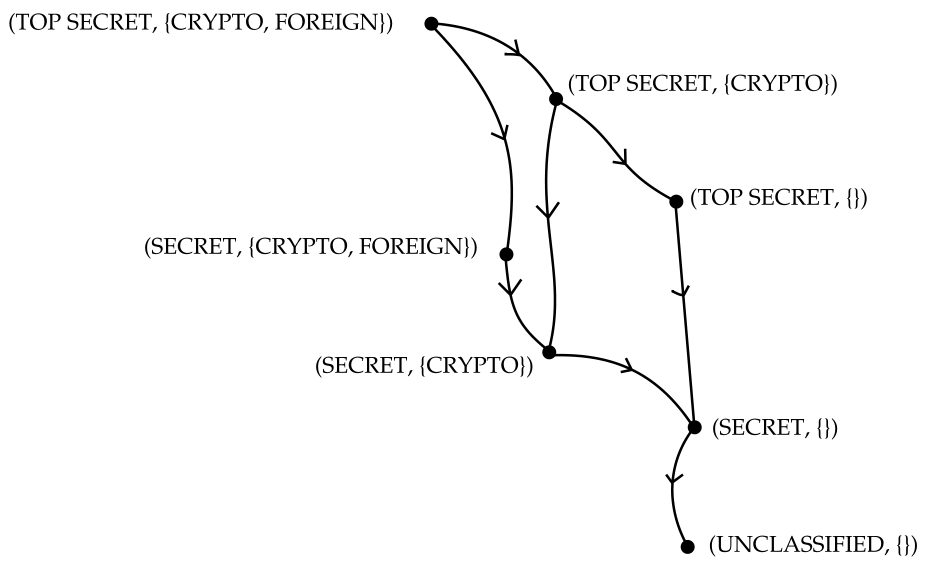
\includegraphics[width=\textwidth]{graphics/blp_lattice}
\end{frame}

\begin{frame}
  \frametitle{Chinese Wall}

  \begin{columns}
    \begin{column}{.33\textwidth}
      \includegraphics[height=.3\textheight]{graphics/chineseSituation}
    \end{column}
    \begin{column}{.33\textwidth}
      \includegraphics[height=.3\textheight]{graphics/chineseChoice1}
    \end{column}
    \begin{column}{.33\textwidth}
      \includegraphics[height=.3\textheight]{graphics/chineseChoice2}
    \end{column}
  \end{columns}
\end{frame}

\begin{frame}
  \frametitle{Decentralized Label Model}

  [insert more simplerer figure]
\end{frame}

\begin{frame}
  \frametitle{Decentralized Label Model \\
    Example}
  \centering

  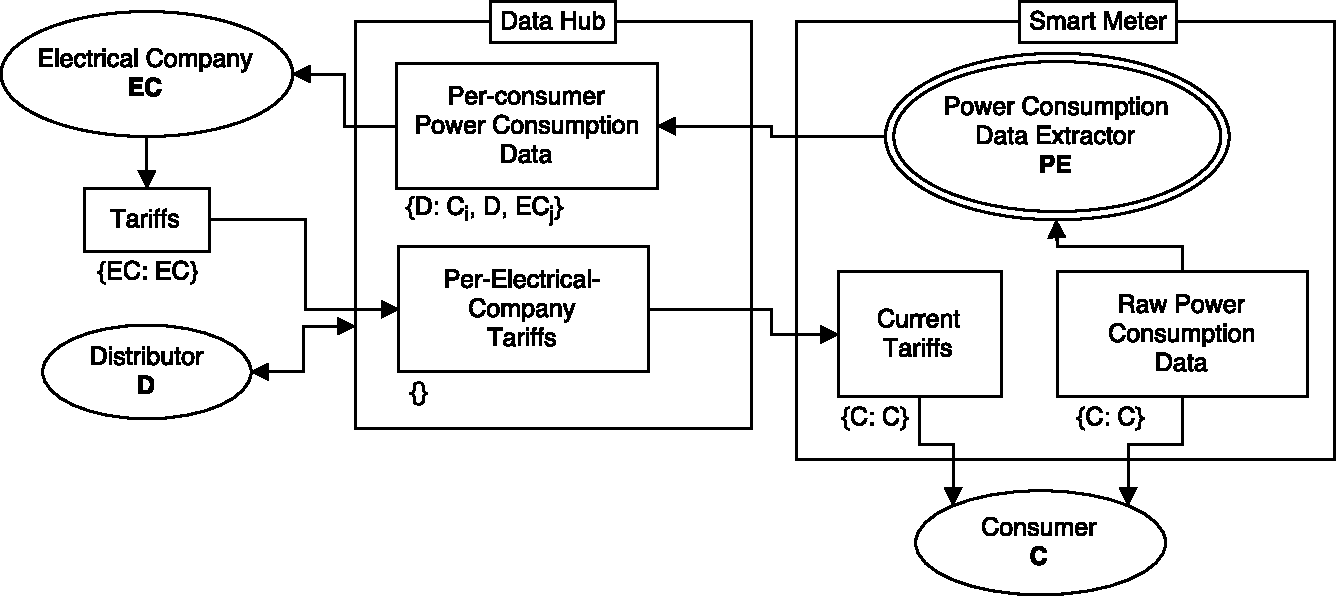
\includegraphics[width=\textwidth]{graphics/dlm_sm_example}
\end{frame}
